% CONTINUES: proof of the corollary \(\psi\bigl(x,L(x)^{c}\bigr)=x\,L(x)^{-\frac1{2c}(1+o(1))}\)
% --- page 50 ---

Since \(B=L(x)^{c}\),
\[
    u=\frac{\log x}{\log B}
     =\frac1c\sqrt{\frac{\log x}{\log\log x}}.
\]
The theorem gives \(\psi(x,B)=x\,u^{-u(1+o(1))}\). Set \(T=u^{-u(1+o(1))}\), so
\(\log T=-u\log u\,(1+o(1))\). From the formula for \(u\),
\[
    \log u
    =\frac12\bigl(\log\log x-\log\log\log x\bigr)-\log c,
\]
and therefore
\begin{align*}
    \log T
    &=-\frac1c\sqrt{\frac{\log x}{\log\log x}}
      \Biggl(\frac12\bigl(\log\log x-\log\log\log x\bigr)-\log c\Biggr)
      (1+o(1))\\
    &=-\frac1{2c}\Biggl(
        \sqrt{\log x\,\log\log x}
        -\sqrt{\frac{\log x}{\log\log x}}\,\log\log\log x
        -2\log c\sqrt{\frac{\log x}{\log\log x}}
      \Biggr)(1+o(1)).
\end{align*}
% FIX p.50: the handwritten third summand is grouped as \((\log c)/c\) inside the
% factor \(1/(2c)\). The expansion of \(\log u\) puts the coefficient \(2\log c\)
% on that summand instead. It is \(o(\log L(x))\) either way.
The first summand is \(\log L(x)\), and the other two are of strictly smaller
order, so
\[
    \log T
    =-\frac1{2c}\log L(x)\,(1+o(1))(1+o(1))
    =-\frac1{2c}\log L(x)\,(1+o(1)).
\]
Hence \(T=L(x)^{-\frac1{2c}(1+o(1))}\), which is the corollary
\[
    \psi\bigl(x,L(x)^{c}\bigr)
    =x\,L(x)^{-\frac1{2c}(1+o(1))}.
    \qedhere
\]
\end{proof}

\begin{keybox}
\begin{theorem}
For \(N\) sufficiently large, and with smoothness bound
\(B=L(N)^{1/\sqrt{2}}\), one expects to test about \(L(N)^{\sqrt{2}}\)
integers in order to find \(\pi(B)+1\) integers that are \(B\)-smooth.
\end{theorem}
\end{keybox}

In particular, this count is subexponential in \(\log N\), and it is the
basis of a subexponential algorithm for factoring \(N\).

% --- page 51 ---
\lectureheading{Lecture 20 (27/10/26)}

\section{Numbers with small prime factors}

The same estimates are restated and proved in this lecture.
Recall
\[
    L(x)=\exp\bigl(\sqrt{\log x\,\log\log x}\bigr),
\]
and write \(o(1)\) for a function of \(x\) that tends to \(0\) as \(x\to\infty\).

\begin{corollary}
For every fixed \(c\) with \(0<c<1\),
\[
    \psi\bigl(x,L(x)^{c}\bigr)
    =x\,L(x)^{-\frac1{2c}(1+o(1))}.
\]
\end{corollary}

\begin{theorem}
For \(N\) sufficiently large, and with \(B=L(N)^{1/\sqrt{2}}\), one expects
to test about \(L(N)^{\sqrt{2}}\) integers in order to find \(\pi(B)+1\)
integers that are \(B\)-smooth.
\end{theorem}

\begin{proof}
The proportion of residues modulo \(N\) that are \(B\)-smooth is
\[
    \frac{\psi(N,B)}{N}.
\]
A \(B\)-smooth residue is useful for the factoring method below once it
is known for about \(\pi(B)+1\) many arguments (one more relation than
there are primes up to \(B\)). The number of random residues one expects
to test is therefore
\[
    \frac{\pi(B)+1}{\psi(N,B)/N}.
\]
The prime-number theorem gives \(\pi(B)\sim B/\log B\) as \(B\to\infty\).
For the one-parameter family \(B=L(N)^{c}\) the corollary supplies
\[
    \frac{\psi(N,B)}{N}
    =L(N)^{-\frac1{2c}(1+o(1))},
\]
and \(\log B=c\log L(N)\), so \(B/\log B=L(N)^{c}/(c\log L(N))\).

% --- page 52 ---
Hence, for \(B=L(N)^{c}\), the expected number of trials is
\begin{align*}
    \frac{\pi(B)+1}{\psi(N,B)/N}
    &=\frac{L(N)^{c}}{c\log L(N)}
      \cdot L(N)^{\frac1{2c}(1+o(1))}\\
    &\approx\frac{L(N)^{c+\frac1{2c}}}{c\log L(N)}.
\end{align*}
The exponent \(f(x)=x+\frac1{2x}\) for \(x>0\) is the quantity to minimise.
Its derivative is \(f'(x)=1-\frac1{2x^{2}}\), so the only positive critical
point is \(x=\frac1{\sqrt{2}}\). Since \(f'(x)<0\) on \(\bigl(0,\frac1{\sqrt{2}}\bigr)\)
and \(f'(x)>0\) on \(\bigl(\frac1{\sqrt{2}},\infty\bigr)\), this critical point
is a minimum.
% FIX p.52: the notes say ``check that this has a minimum'' without writing
% the derivative. The one-line computation of \(f'\) is filled in.

\begin{figure}[H]
\centering
\begin{tikzpicture}[scale=1.35]
    \draw[->] (0.30,0.95) -- (2.55,0.95) node[right] {\(x\)};
    \draw[->] (0.30,0.95) -- (0.30,2.85) node[above] {\(f(x)\)};
    \draw[domain=0.36:2.40,samples=80,smooth,thick] plot (\x,{\x+1/(2*\x)});
    \draw[dashed] (0.7071,0.95) -- (0.7071,1.4142);
    \fill (0.7071,1.4142) circle (1.7pt);
    \node[below] at (0.7071,0.92) {\(\dfrac{1}{\sqrt{2}}\)};
\end{tikzpicture}
\caption{The function \(f(x)=x+\frac1{2x}\), with its minimum marked at
\(x=1/\sqrt{2}\).}
\end{figure}

Take \(c=\frac1{\sqrt{2}}\). Then
\[
    c+\frac1{2c}
    =\frac1{\sqrt{2}}+\frac1{\sqrt{2}}
    =\sqrt{2},
\]
because \(\frac1{2c}=\frac{\sqrt{2}}{2}=\frac1{\sqrt{2}}\). The expected
number of trials is therefore about
\[
    \frac{L(N)^{\sqrt{2}}}{c\log L(N)}.
\]
The denominator grows much more slowly than every positive power of
\(L(N)\), so the count is \(L(N)^{\sqrt{2}\,(1+o(1))}\), which is the
statement of the theorem (and \(B=L(N)^{c}=L(N)^{1/\sqrt{2}}\)).
\end{proof}

\subsection{Generating the smooth values}
\label{sec:sieving-idea}

The integers that have to be produced are not arbitrary. One wants many
integers \(a>\sqrt{N}\) such that \(a^{2}\bmod N\) is \(B\)-smooth. Those
residues are generated by a sieve rather than by trial division of each
candidate.

% --- page 53 ---

\begin{figure}[H]
\centering
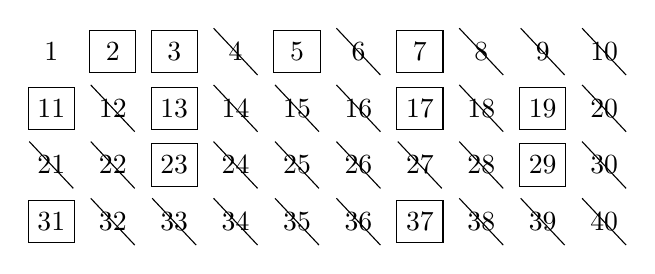
\begin{tikzpicture}[x=0.78cm,y=0.72cm]
    \foreach \n in {1,...,40} {
        \pgfmathtruncatemacro{\c}{mod(\n-1,10)}
        \pgfmathtruncatemacro{\r}{int((\n-1)/10)}
        \node[minimum width=1.35em,minimum height=1.25em,inner sep=1pt]
            (s\n) at (\c,-\r) {\(\n\)};
    }
    \foreach \p in {2,3,5,7,11,13,17,19,23,29,31,37} {
        \draw ([shift={(-1.4pt,1.2pt)}]s\p.north west)
              rectangle
              ([shift={(1.4pt,-1.2pt)}]s\p.south east);
    }
    \foreach \m in {4,6,8,9,10,12,14,15,16,18,20,21,22,24,25,26,27,28,30,32,33,34,35,36,38,39,40} {
        \draw ([shift={(-1pt,2pt)}]s\m.north west)
              --
              ([shift={(1pt,-2pt)}]s\m.south east);
    }
\end{tikzpicture}
\caption{Sieve of Eratosthenes on \(\{1,\ldots,40\}\). Primes are boxed and
composite numbers are struck out. The entry \(1\) is neither.}
\end{figure}

List a run of integers and strike out multiples of primes, and of prime
powers, in increasing order, keeping only prime powers that are at most
the smoothness bound \(B\). What survives is \(B\)-smooth.

\subsection{The quadratic sieve}
\label{sec:qs}

The quadratic sieve (Pomerance) turns the same idea into a factoring
algorithm. The goal is to find an integer \(a\) such that \(a^{2}\bmod N\)
is \(B\)-smooth.

Start from the polynomial \(F(t)=t^{2}-N\). List the values
\[
    F(a),\; F(a+1),\; \ldots,\; F(b),
\]
where \(a=\lfloor\sqrt{N}\rfloor+1\) and the right endpoint \(b\) is large
enough that the list contains about \(L(N)^{\sqrt{2}}\) entries. An entry
is \(B\)-smooth precisely when every prime dividing it is at most \(B\).

For an odd prime \(p\le B\), the congruence \(t^{2}-N\equiv 0\pmod{p}\)
has either no solution or two solutions modulo \(p\). If \(\alpha_{p}\) and
\(\beta_{p}\) are the two solutions, then every integer in either of the
arithmetic progressions
\[
    \alpha_{p}+p,\;\alpha_{p}+2p,\;\alpha_{p}+3p,\;\ldots
    \qquad\text{and}\qquad
    \beta_{p}+p,\;\beta_{p}+2p,\;\beta_{p}+3p,\;\ldots
\]
is likewise a solution. At each such argument, \(p\) divides \(F(t)\), so
the sieve can divide the whole progression by \(p\) (and by the prime
powers \(p^{e}\le B\)) in one pass.

% --- page 54 ---

\begin{example}[Sieving \(F(t)=t^{2}-221\)]
Let \(N=221\). Then \(\sqrt{N}\approx 14.9\), so the list begins at
\(t=15\):
\[
    F(t)=t^{2}-N,\qquad t=15,16,17,\ldots.
\]
Dividing by \(2\), \(4\), \(5\), and \(7\) along the progressions above
produces the following array. An arrow means that the entry is divisible
by the next prime power and is replaced by the quotient.

\begin{figure}[H]
\centering
\setlength{\tabcolsep}{5.5pt}
\renewcommand{\arraystretch}{1.18}
\begin{tabular}{l|cccccccc}
    & \(15\) & \(16\) & \(17\) & \(18\) & \(19\) & \(20\) & \(21\) & \(22\) \\
    \hline
    \(F(t)\)
        & \(4\) & \(35\) & \(68\) & \(103\) & \(140\) & \(179\) & \(220\) & \(263\) \\
        & \(\downarrow\) & & \(\downarrow\) & & \(\downarrow\) & & \(\downarrow\) & \\
    divide by \(2\)
        & \(2\) & & \(34\) & & \(70\) & & \(110\) & \\
        & \(\downarrow\) & & \(\downarrow\) & & \(\downarrow\) & & \(\downarrow\) & \\
    divide by \(4\)
        & \(1\) & & \(17\) & & \(35\) & & \(55\) & \\
        & & \(\downarrow\) & & & \(\downarrow\) & & \(\downarrow\) & \\
    divide by \(5\)
        & & \(7\) & & & \(7\) & & \(11\) & \\
        & & \(\downarrow\) & & & \(\downarrow\) & & & \\
    divide by \(7\)
        & & \(1\) & & & \(1\) & & & \\
\end{tabular}
\caption{Quadratic sieve for \(N=221\) on \(t=15,\ldots,22\). Blank cells
are not divisible by that prime power. A final entry \(1\) means that
\(F(t)\) factored completely over \(\{2,5,7\}\).}
\end{figure}

The prime \(p=3\) never occurs. Indeed
\[
    221\equiv 2\pmod{3},
\]
and \(2\) is not a square modulo \(3\), so \(t^{2}\equiv 221\pmod{3}\) has
no solution and the progression for \(p=3\) is empty.

\begingroup\samepage
Reading off the rows that reach \(1\), together with the two further
arguments \(t=21\) and \(t=23\) whose cofactor is the prime \(11\),
\begin{align*}
    15^{2}-N &= 2^{2},\\
    16^{2}-N &= 5\cdot 7,\\
    19^{2}-N &= 2^{2}\cdot 5\cdot 7,\\
    21^{2}-N &= 2^{2}\cdot 5\cdot 11,\\
    23^{2}-N &= 2^{2}\cdot 7\cdot 11.
\end{align*}
\endgroup
% FIX p.54: \(23^{2}-221=308=2^{2}\cdot 7\cdot 11\). A first reading of the
% exponent of \(2\) is ambiguous; the integer factorisation forces \(2^{2}\).
The second and third relations multiply to a square on both sides:
\[
    (5\cdot 7)\cdot(2^{2}\cdot 5\cdot 7)
    =(2\cdot 5\cdot 7)^{2},
\]
so
\[
    (16\cdot 19)^{2}\equiv(2\cdot 5\cdot 7)^{2}\pmod{N}.
\]
Set \(a=16\cdot 19=304\) and \(b=70\). Then \(a-b=234\), and
\[
    \gcdop(234,221)=13.
\]
Thus \(N=13\cdot 17\).
\end{example}

% --- page 55 ---

The same list contains a second dependency, and it is useless. Multiplying
the relations for \(t=16\), \(21\), and \(23\) gives exponents
\(2^{4}\cdot 5^{2}\cdot 7^{2}\cdot 11^{2}\), hence
\[
    (16\cdot 21\cdot 23)^{2}
    \equiv(2^{2}\cdot 5\cdot 7\cdot 11)^{2}\pmod{N}.
\]
Here \(a=16\cdot 21\cdot 23=7728\) and \(b=2^{2}\cdot 5\cdot 7\cdot 11=1540\), so
\begin{align*}
    \gcdop(a-b,N)&=\gcdop(6188,221)=221,\\
    \gcdop(a+b,N)&=\gcdop(9268,221)=1.
\end{align*}
Both greatest common divisors are trivial factors of \(N\).

\begin{remark}
Let \(p\) be an odd prime and let \(e\ge 1\). In the situation used by the
sieve, where \(p\) does not divide \(N\), the congruence
\[
    t^{2}\equiv N\pmod{p^{e}}
\]
has either no solution or exactly two solutions.
% FIX p.55: the notes omit the hypothesis that \(p\) does not divide \(N\).
% Without it the count of solutions can fail (for instance if \(p\) divides \(N\)).
\end{remark}

Concretely, before a prime \(p\) is used in the sieve one has to decide
whether \(N\) is a square modulo \(p\). For \(N=221\) and \(p=3\) it is not,
as above.

Quadratic residuosity is not only a sieving test. The distinction between
quadratic residues and quadratic non-residues can be used as the hidden
bit of a public-key encryption scheme, the Goldwasser--Micali cryptosystem.

If the plaintext were a bare bit \(m\in\{0,1\}\) and the encryption map
were deterministic, an eavesdropper would recognise \(m\) just by comparing
a ciphertext with the two possible encryptions. The way around this is to
pad the bit with randomness: replace \(m\) by a pair \((m,x)\) that is
sufficiently random, and encrypt the pair.

% --- page 56 ---

\section{The Goldwasser--Micali cryptosystem}
\label{sec:gm}

\paragraph{Key generation.}
Alice chooses two primes \(p\) and \(q\), and an integer \(a\) with
\[
    \Bigl(\frac{a}{p}\Bigr)=-1
    \qquad\text{and}\qquad
    \Bigl(\frac{a}{q}\Bigr)=-1.
\]
She publishes the modulus \(N=pq\) and the quadratic non-residue \(a\), and
she keeps the factorization \((p,q)\).

\paragraph{Encryption.}
Bob wants to send a bit \(m\in\{0,1\}\). He chooses an integer \(x\) with
\(1<x<N\) at random and sends
\[
    c\equiv
    \begin{cases}
        x^{2}\pmod{N} & \text{if }m=0,\\
        ax^{2}\pmod{N} & \text{if }m=1.
    \end{cases}
\]

\paragraph{Decryption.}
Alice receives \(c\) and computes the Legendre symbols
\(\bigl(\frac{c}{p}\bigr)\) and \(\bigl(\frac{c}{q}\bigr)\). For the symbol
modulo \(p\), and assuming \(\gcdop(x,N)=1\),
\[
    \Bigl(\frac{c}{p}\Bigr)
    =
    \begin{cases}
        \Bigl(\dfrac{x^{2}}{p}\Bigr)
            =\Bigl(\dfrac{x}{p}\Bigr)^{2}
            =1 & \text{if }m=0,\\[1.6em]
        \Bigl(\dfrac{ax^{2}}{p}\Bigr)
            =\Bigl(\dfrac{a}{p}\Bigr)\Bigl(\dfrac{x}{p}\Bigr)^{2}
            =-1 & \text{if }m=1.
    \end{cases}
\]
The same computation modulo \(q\) gives
\[
    \Bigl(\frac{c}{q}\Bigr)
    =
    \begin{cases}
        1 & \text{if }m=0,\\
        -1 & \text{if }m=1.
    \end{cases}
\]
Either symbol is therefore \((-1)^{m}\), and Alice recovers the bit.

\paragraph{What Eve sees.}
Eve knows \(N\), \(a\), and \(c\), and she can form the Jacobi symbol
\(\bigl(\frac{c}{N}\bigr)\). In both cases the value lies in \(\{1,0\}\):
\[
    \Bigl(\frac{c}{N}\Bigr)
    =
    \begin{cases}
        \Bigl(\dfrac{x^{2}}{N}\Bigr)
            =\Bigl(\dfrac{x}{N}\Bigr)^{2}
            \in\{1,0\} & \text{if }m=0,\\[1.6em]
        \Bigl(\dfrac{ax^{2}}{N}\Bigr)
            =\Bigl(\dfrac{x}{N}\Bigr)^{2}\Bigl(\dfrac{a}{pq}\Bigr)
            =\Bigl(\dfrac{x}{N}\Bigr)^{2}
            \underbrace{\Bigl(\dfrac{a}{p}\Bigr)\Bigl(\dfrac{a}{q}\Bigr)}_{=\,1}
            \in\{1,0\} & \text{if }m=1.
    \end{cases}
\]
The symbol equals \(1\) when \(\gcdop(x,N)=1\) and equals \(0\) when \(p\) or
\(q\) divides \(x\). It is never \(-1\), so it does not reveal the bit.
The factorization of \(N\) is what makes the two Legendre symbols available
to Alice.

% --- page 57 ---

\begin{remark}
The scheme as written is not practical: each ciphertext, a number modulo
\(N\), carries a single bit of message.
\end{remark}

\section{Index calculus}
\label{sec:index-calculus}

Index calculus is a subexponential algorithm for the discrete logarithm
problem in \(\units{p}\). Recall from Lecture~12 that the problem is: given a prime \(p\), a primitive
root \(g\) modulo \(p\), and a target \(h\in\units{p}\), find the integer
\(x\) with \(1\le x\le p-1\) and
\[
    g^{x}\equiv h\pmod{p}.
\]
That integer is \(x=\ind_{g}(h)\).

Instead of attacking \(h\) directly, first solve
\[
    g^{x}\equiv \ell\pmod{p}
\]
for every prime \(\ell\le B\), for a smoothness bound \(B\) still to be
chosen. The solutions are the factor-base logarithms \(\ind_{g}(\ell)\).

The individual logarithm is then a search for one further smooth value.
Compute \(hg^{k}\bmod p\) for \(k=1,2,3,\ldots\) until the residue is
\(B\)-smooth, say
\[
    hg^{k}
    \equiv\prod_{\ell\le B}\ell^{e_{\ell}}\pmod{p}.
\]
Taking \(\ind_{g}\) of both sides yields the linear congruence
\[
    \ind_{g}(h)+k
    \equiv\sum_{\ell\le B}e_{\ell}\,\ind_{g}(\ell)
    \pmod{p-1},
\]
and therefore
\[
    \ind_{g}(h)
    \equiv -k+\sum_{\ell\le B}e_{\ell}\,\ind_{g}(\ell)
    \pmod{p-1}.
\]

\lectureheading{Lecture 21 (30/10/26)}

% --- page 58 ---

The missing ingredient is the computation of \(\ind_{g}(\ell)\) for the
primes \(\ell\le B\). Draw exponents \(i\ge 1\) at random and set
\[
    g_{i}\equiv g^{i}\pmod{p}.
\]
Whenever \(g_{i}\) is \(B\)-smooth, write
\[
    g_{i}=\prod_{\ell\le B}\ell^{e_{\ell}(i)}
\]
in \(\Z\), up to the representative chosen modulo \(p\). Then
\[
    \ind_{g}(g_{i})
    \equiv\sum_{\ell\le B}e_{\ell}(i)\,\ind_{g}(\ell)
    \pmod{p-1},
\]
and since \(\ind_{g}(g_{i})\equiv i\pmod{p-1}\),
\[
    i\equiv\sum_{\ell\le B}e_{\ell}(i)\,\ind_{g}(\ell)
    \pmod{p-1}.
\]
Each smooth \(g_{i}\) is one linear equation in the unknowns
\(\ind_{g}(\ell)\), \(\ell\le B\). Enough such equations determine those
unknowns.

The modulus of the system is \(p-1\). By the Chinese Remainder Theorem it
is enough to solve the system modulo \(q^{\alpha}\) for each prime power
\(q^{\alpha}\) in the factorization of \(p-1\): solve first modulo \(q\),
then lift the solution to \(q^{\alpha}\).

The smooth-number count of the previous lecture applies with \(x=p\).
If the factor base is cut at
\[
    B=L(p)^{1/\sqrt{2}},
\]
one expects to test about \(L(p)^{\sqrt{2}}\) exponents \(i\) before
enough relations have been found.

As in the quadratic sieve, the relations should be collected by a sieve.
Rather than factoring each \(g^{i}\bmod p\) from scratch, list the
candidates and divide by primes and prime powers wherever the
corresponding congruence permits it.

% --- page 59 ---

\begin{example}[A small index calculus]
\label{ex:index}
Let \(p=232487\), and take \(g=229401\) and \(h=171020\). The problem is
to solve \(g^{x}\equiv h\pmod{p}\).

Take the smoothness bound \(B=7\), so the factor base is
\(\{2,3,5,7\}\). Four smooth relations are
\begin{align*}
    g^{482}&\equiv 2^{5}\cdot 3^{2}\cdot 7^{3}\pmod{p},\\
    g^{600}&\equiv 2^{2}\cdot 3^{9}\pmod{p},\\
    g^{876}&\equiv 2^{9}\cdot 3^{4}\pmod{p},\\
    g^{948}&\equiv 2^{6}\cdot 5^{2}\pmod{p}.
\end{align*}
Write \(x_{i}=\ind_{g}(i)\) for \(i\in\{2,3,5,7\}\). The relations become
the linear system
\begin{align*}
    482&\equiv 5x_{2}+2x_{3}+3x_{7},\\
    600&\equiv 2x_{2}+9x_{3},\\
    876&\equiv 9x_{2}+4x_{3},\\
    948&\equiv 6x_{2}+2x_{5},
\end{align*}
which the notes record modulo \((p-1)/2\). Each congruence is an equality
of indices, so it holds modulo \(p-1\) as well. The modulus factors as
\(p-1=232486=2\cdot 116243\). Reducing modulo \(2\) gives
\begin{align*}
    x_{2}+x_{7}&\equiv 0\pmod{2},\\
    x_{3}&\equiv 0\pmod{2},\\
    x_{2}&\equiv 0\pmod{2},
\end{align*}
while the last equation is \(0\equiv 0\pmod{2}\) and does not constrain
\(x_{5}\). Therefore
\[
    x_{2}\equiv x_{3}\equiv x_{7}\equiv 0\pmod{2},
\]
and \(x_{5}\) may be either even or odd.

Solving the original system modulo \((p-1)/2=116243\) produces one
solution class
\begin{align*}
    x_{2}&\equiv 38292,\\
    x_{3}&\equiv 30305,\\
    x_{5}&\equiv 1841,\\
    x_{7}&\equiv 71128,
\end{align*}
all modulo \((p-1)/2\).

% --- page 60 ---
The parity conditions select the lifts of \(x_{2}\), \(x_{3}\), and
\(x_{7}\). The representatives \(38292\) and \(71128\) are already even,
while \(30305\) is odd, so
\begin{align*}
    x_{2}&\equiv 38292,\\
    x_{3}&\equiv 30305+116243=146548,\\
    x_{7}&\equiv 71128,
\end{align*}
modulo \(p-1\). For \(x_{5}\) the coefficient in the system is even, so
both lifts satisfy the congruences. The power
\[
    g^{1841}\equiv 5\pmod{p}
\]
selects \(x_{5}\equiv 1841\pmod{p-1}\).
% The notes cross out a side product \(117\times 84\) between
% \(x_{5}\equiv 1841\) and \(5=g^{1841}\pmod{p}\). It is not used.

A further smooth multiple of the target is
\[
    g^{166}\cdot h\equiv 2^{7}\cdot 3^{2}\cdot 5^{2}\cdot 7\pmod{p}.
\]
Taking indices,
\[
    166+\ind_{g}(h)
    \equiv 7x_{2}+2x_{3}+2x_{5}+x_{7}
    \pmod{p-1}.
\]
The right-hand side evaluates to
\begin{align*}
    7\cdot 38292+2\cdot 146548+2\cdot 1841+71128
    &=635950\\
    &=2(p-1)+170978,
\end{align*}
so
\[
    \ind_{g}(h)
    \equiv 170978-166
    =170812\pmod{p-1}.
\]
% The notes record the result \(170812\) without the intermediate sum.
% The arithmetic above is that skipped evaluation.
Thus \(g^{170812}\equiv h\pmod{p}\).
\end{example}

Index calculus solves the discrete logarithm problem in \(\units{p}\) in
subexponential time.

\section{Elliptic Curves}
\label{sec:ec-warmup}

Discrete logarithms on elliptic curves, by contrast,
require exponential time with the algorithms available for a general curve.

\subsection{Warm-up: rational points on the circle}

Consider the circle \(C\colon x^{2}+y^{2}=1\).

\begin{figure}[H]
\centering
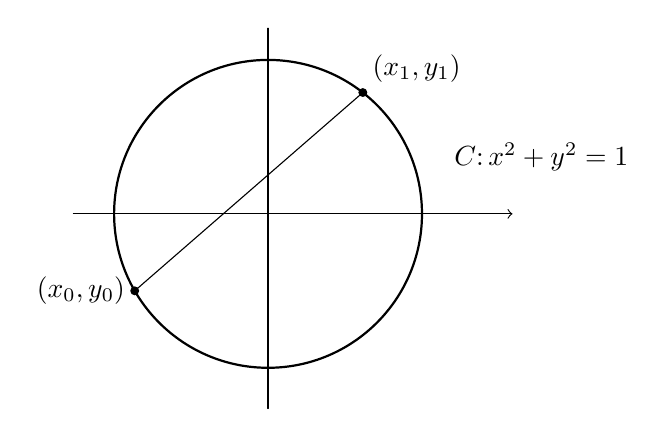
\begin{tikzpicture}[scale=1.15,line cap=round]
    \draw[thick] (0,0) circle (1.7);
    \draw[->] (-2.15,0) -- (2.7,0);
    \draw (0,-2.15) -- (0,2.05);
    \coordinate (P0) at (210:1.7);
    \coordinate (P1) at (52:1.7);
    \draw (P0) -- (P1);
    \fill (P0) circle (1.4pt);
    \fill (P1) circle (1.4pt);
    \node[left] at (P0) {\((x_{0},y_{0})\)};
    \node[above right] at (P1) {\((x_{1},y_{1})\)};
    \node[anchor=west] at (18:2.05) {\(C\colon x^{2}+y^{2}=1\)};
\end{tikzpicture}
\caption{The circle \(C\colon x^{2}+y^{2}=1\), with a chord through two of
its points.}
\end{figure}

The aim is to study the points of this curve, then to study them by means
of a parameter, and in particular to study the rational points by means of
a rational parameter.

% --- page 61 ---

A point is rational when it lies in \(\mathbb{Q}^{2}\). The integer points
on \(C\) are
\[
    \bigl\{(\pm 1,0),\,(0,\pm 1)\bigr\}.
\]
There are many further rational points, for instance
\[
    \Bigl(\frac{3}{5},\frac{4}{5}\Bigr),
    \qquad
    \Bigl(\frac{5}{13},\frac{12}{13}\Bigr),
    \qquad\ldots,
\]
coming from primitive Pythagorean triples.

\begin{claim}
Let \((x_{0},y_{0})\) and \((x_{1},y_{1})\) be rational points of \(C\).
The line through them has rational slope.
\end{claim}

Conversely, start with one rational point \((x_{0},y_{0})\) and a rational
slope \(t\). The line of slope \(t\) through \((x_{0},y_{0})\) meets \(C\)
again at a point \((x_{1},y_{1})\). That second point is rational: already
\(x_{1}\in\mathbb{Q}\), or equivalently \(y_{1}\in\mathbb{Q}\), and
therefore \((x_{1},y_{1})\in\mathbb{Q}^{2}\).

Take the base point to be \((x_{0},y_{0})=(-1,0)\). The line of slope \(t\)
through this point is \(y=t(x+1)\). It meets the tangent line \(x=1\) at
the point \((1,2t)\), which is the picture used to solve for the second
intersection with the circle.

\begin{figure}[H]
\centering
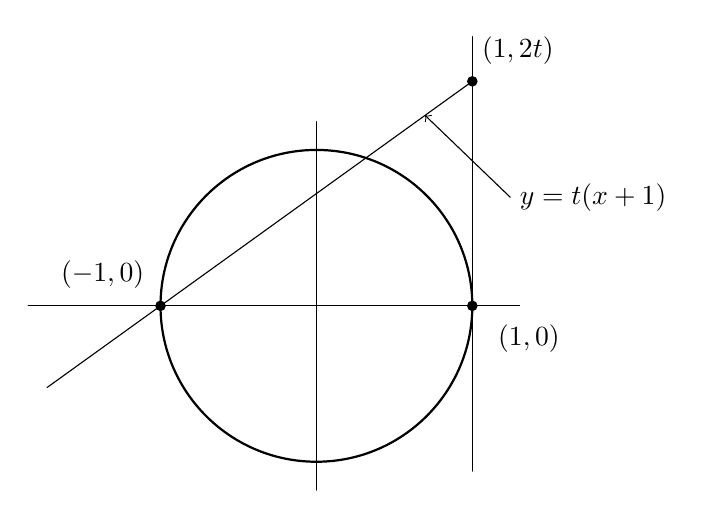
\begin{tikzpicture}[scale=1.2,line cap=round]
    \draw[thick] (0,0) circle (1.65);
    \draw (-3.05,0) -- (2.15,0);
    \draw (0,-1.95) -- (0,1.95);
    % unit circle scaled by 1.65; the line x=1 is tangent at (1,0)
    \draw (1.65,-1.75) -- (1.65,2.85);
    % y=t(x+1) with t=0.72; picture height of (1,2t) is 2*0.72*1.65
    \draw (-2.85,-0.864) -- (1.65,2.376);
    \fill (-1.65,0) circle (1.6pt);
    \node[above left] at (-1.72,0.08) {\((-1,0)\)};
    \fill (1.65,0) circle (1.6pt);
    \node[anchor=north west] at (1.82,-0.10) {\((1,0)\)};
    \fill (1.65,2.376) circle (1.6pt);
    \node[above right] at (1.65,2.45) {\((1,2t)\)};
    \node[anchor=west] (eq) at (2.05,1.15) {\(y=t(x+1)\)};
    \draw[->] (eq.west) -- (1.15,2.016);
\end{tikzpicture}
\caption{The line \(y=t(x+1)\) through \((-1,0)\). It meets the tangent
line \(x=1\) at \((1,2t)\).}
\end{figure}
